
\documentclass[11pt]{article}
\usepackage{amsmath,textcomp,amssymb,graphicx,cancel}
\usepackage{gensymb}
\usepackage[margin=1in]{geometry}
\usepackage{pgfplots}
\pgfplotsset{width=7cm,compat=1.8}
\usepackage[colorlinks, urlcolor=blue]{hyperref}
\usepackage{tikz}
\usepackage{epigraph}

%\setlength\parindent{24pt}

\def\Name{Zackery Field}  % Your name
\def\Session{Fall 2013} %Semester

\title{BIOE147 -- Fall 2013 -- PS3}
\author{\Name}
\markboth{BIOE147 \Session \Name}{\Name -- PS3}
\pagestyle{myheadings}

\renewcommand\epigraphflush{flushright}
\renewcommand\epigraphsize{\normalsize}
\setlength\epigraphwidth{0.7\textwidth}

\definecolor{titlepagecolor}{cmyk}{1,.60,0,.40}

\begin{document}

\maketitle
\section*{1. Stability}
 
{\centering
  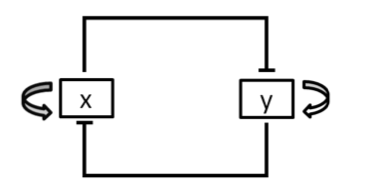
\includegraphics[scale=0.75, trim = 0mm 0mm 7mm 0mm, clip]{ps3_stability.png}\par
 }
\begin{itemize}

\item $x$ activates further production of $x$ at a rate $\frac{k_1x^n}{k_2+x^n}$
\item $y$ activates further production of $y$ at a rate $\frac{k_4y^m}{k_5+y^m}$
\item $x$ and $y$ bind each other in a bimolecular interaction to form a dead end complex with rate constant $k_3$.

\item[] Differential equations for x and y:

\begin{equation*}
  \begin{align}
    \frac{d[x]}{dt} = \frac{k_1[x]^n}{k_2+[x]^n} - k_3[x][y]\\
    \frac{d[y]}{dt} = \frac{k_4[y]^m}{k_5+[y]^m} - k_3[x][y]
  \end{align}
\end{equation}

\item[]Sketch of nullclines for $x$ and $y$ if $n=m=4$:


{
 \centering
  \begin{tikzpicture}
    \begin{axis}%
      [
        height = 7cm,
        width = 7cm,
        xlabel ={[x]},
        ylabel ={[y]},
        xticklabels={,,},
        yticklabels={,,}
      ]
      \addplot%
          [
            blue,%
            mark=none,
            samples=100,
            domain=-6:6
          ]
          (x+2,{1-(1/(1+exp(-(1.75)*x)))-.3});
          \addlegendentry{$x$};
          
          \addplot%
              [
                red,%
                mark=none,
                samples=100,
                domain=-6:6
              ]
              (x,{1 - 1/(1+exp(-1.75*x))/.8});
              \addlegendentry{$y$};
    \end{axis}
  \end{tikzpicture}
}


\item[] Graph the nullclines and velocity plots using the following sets of parameters:

I ran into a number of issues making the velocity plots on MATLAB.

\item[] Does the circuit perform like a toggle switch in any of the simulated parameter sets? 

see above.

\item[] What values for which parameters promote multiple steady states? Why? Which steady states
are stable?

The parameters that lead to multiple steady states include two interesecting nullcline points.
This is pictured in the sketch above. These nullcline points represent where the change in 
[x] and [y] both pull towards the these intersecting points. Any fluctuation would cause a push back
to these steady state points.        

\end{itemize}
\newpage 

\section*{2. Feedforward and feedback}


{\centering
  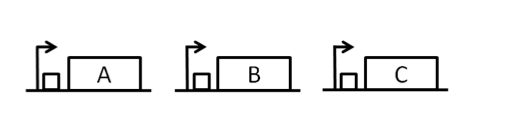
\includegraphics[scale=0.75, trim = 0mm 0mm 7mm 0mm, clip]{ps3_q2.png}\par
 }
\begin{itemize}
\item[] Hook up the above transcription units into a feedforward pulse generator that responds to step increases in A. 
Write differential equations for rate changes in proteins A, B, and C and in other relevant species. 

Assume that the initial input I acts on the operator of A, A acts on the operator of B, B acts on the operator of C, and
C is the output signal. 
As the problem states, this system will respond to step increases in A, but for completeness 
the step changes in A will be induced by the presence of I.  
This condition is sufficient to describe a feedforward system. An example of this type of system is in 
E. coli whereby the presence of a collection of initial inputs will initiate genomic replication.  

\begin{equation*}
  \begin{align}
    \frac{d[A]}{dt} &= \frac{k_1[I]^n}{k_2+[I]^n} - k_3[A]^m\\
    \frac{d[B]}{dt} &= \frac{k_4[A]^m}{k_5+[A]^m} - k_6[B]^g\\
    \frac{d[C]}{dt} &= \frac{k_7[B]^g}{k_8+[B]^g}\\
  \end{align}
\end{equation*}

\item[] Justify your choice of rate forms for reactions with order 2 or greater. 

The order of the rate forms depend on the values of n, m, and g. The degradation rates of [A] and [B] will also
depend on the order of the first rate form in each of the equations. 

\item[] Do you think you can speed up the response rate by adding negative feedback? Explain or use simulations to prove your point. 

Yes, the response rate should increase with the addition of negative feedback.   

\item[] Is the process reversible (ie. if you take the high A, low C state and remove A will you reset to the low A, low C state)? 

Yes, the process is reversible. Because the high A would be in a negative feedback loop resetting back to low A will reduce C back to low.

\item[] Is there anything peculiar about the dynamics of the reverse process (or lack therof)?

n/a

\item[] Is there a way to hook up the above transcription units to give a transient decrease in C below a high
 basal level when A goes from off to on, without adding additional elements?

n/a

\end{itemize}
\end{document}
